\subsection{LSTM - Long Short Term Memory}

One of two more common solutions to avoid the pitfalls \acrshort{rnn}s give us, is to use \acrshort{lstm} cells. 

 As we've mentioned, regular \acrshort{rnn}s struggle with long term memory, something the \acrshort{lstm} cells solves. \\ 


An \acrshort{lstm} cell is built up by the following components: an input gate $i$, a forget gate $f$, a candidate state $g$, an output gate $g$ .
These cells traditionally make use of the sigmoid non-linearity function $\sigma()$

\begin{figure}[h]
    \centering
    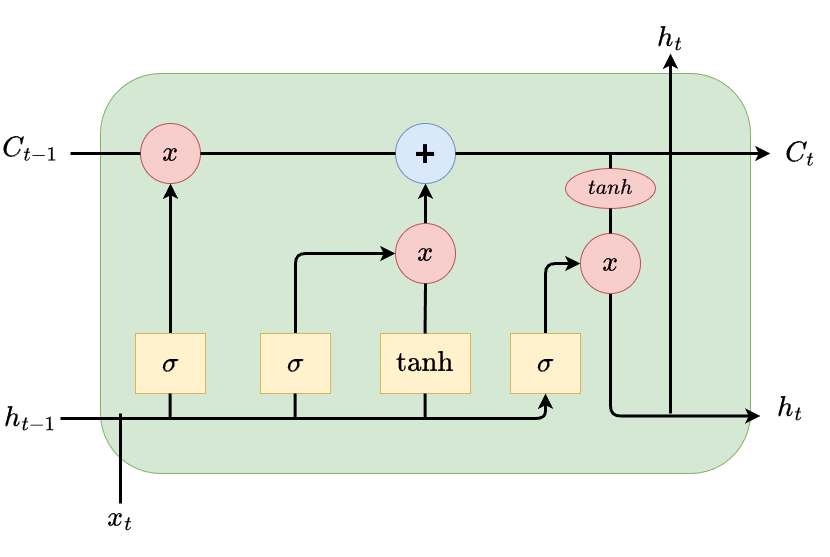
\includegraphics{figures/lstmcell.png}
    \caption[scale=0.4]{Example of an LSTM cell}
    \label{fig:lstmcell}
\end{figure}

Compared to the equation for forward pass 

\begin{equation} \label{eq:cnn}
    Y_t = W_xx_t + b
\end{equation}

the \acrshort{lstm} keeps the previous state in mind, thus giving us the equation


\begin{equation} \label{eq:lstm}
    Y_t = W_hh_{t-1} + W_xx_t + b
\end{equation}

Adding batch normalization to this equation and we end up with the following equation \cite{cooijmans2017recurrent}: 

\begin{equation} \label{eq:bnlstm}

c_t = \sigma(\Tilde{\textbf{f}_t} \cdot c_{t-1} + \sigma(\textbf{\Tilde{i}}_t) \cdot tanh(\Tilde{g}_t)
h_t = \sigma(\Tilde{o}_t) \cdot tanh(BN(\textbf{c_t}; \gamma_c, \beta_c))
    
\end{equation}

By applying batch normalization to \acrshort{lstm}s, not only did the models converge faster, the performance was up to par with the unnormalized \acrshort{lstm} \cite{cooijmans2017recurrent}.

Whereas \acrshort{rnn}s shines at \acrshort{nlp}, speech recognition, and media processing, \acrshort{lstm}s is vastly better for time series forecasting due to the memory gates. This makes \acrshort{lstm}s a suitable option for us when working with anomaly detection on sensor data, which in its essence is nothing more than more complex time series data across multiple columns or channels. 

The alternative to using \acrshort{lstm} nodes for our network would be \acrfull{gru}s.


\subsubsection{Loss functions}

In typical LSTM 

\acrfull{mae} is the most common algorithm when it 

\subsubsection{Activation fun


\subsubsection{Optimizers for Unsupervised Learning }

Diffre



JudasNET uses \Gls{adam} as its optimizer, which is defined as follows: 


\begin{align}
    m_t &= \beta_1 m_{t-1} + (1 - \beta_1) g_t \\
    v_t &= \beta_2 v_{t-1} + (1 - \beta_2) g_t^2 \\
    \hat{m}_t &= \frac{m_t}{1 - \beta_1^t} \\
    \hat{v}_t &= \frac{v_t}{1 - \beta_2^t} \\
    \theta_{t+1} &= \theta_t - \frac{\alpha}{\sqrt{\hat{v}_t} + \epsilon} \hat{m}_t
\end{align}

where:
\begin{align*}
    \theta_t & \text{ - parameters at time step } t \\
    g_t & \text{ - gradient of the loss function at time step } t \\
    \alpha & \text{ - learning rate} \\
    \beta_1, \beta_2 & \text{ - exponential decay rates for the moment estimates} \\
    m_t, v_t & \text{ - first and second moment estimates} \\
    \hat{m}_t, \hat{v}_t & \text{ - bias-corrected first and second moment estimates} \\
    \epsilon & \text{ - small constant to prevent division by zero}
\end{align*}

The original paper sets the following parameters for ADAM: $\beta_1 = 0.99, \beta_2 = 0.9 \mu=10^{-8}$ and $\alpha = 0.001$ \cite{kingma2017adam}.